% Options for packages loaded elsewhere
\PassOptionsToPackage{unicode}{hyperref}
\PassOptionsToPackage{hyphens}{url}
\documentclass[
]{article}
\usepackage{xcolor}
\usepackage[margin=1in]{geometry}
\usepackage{amsmath,amssymb}
\setcounter{secnumdepth}{-\maxdimen} % remove section numbering
\usepackage{iftex}
\ifPDFTeX
  \usepackage[T1]{fontenc}
  \usepackage[utf8]{inputenc}
  \usepackage{textcomp} % provide euro and other symbols
\else % if luatex or xetex
  \usepackage{unicode-math} % this also loads fontspec
  \defaultfontfeatures{Scale=MatchLowercase}
  \defaultfontfeatures[\rmfamily]{Ligatures=TeX,Scale=1}
\fi
\usepackage{lmodern}
\ifPDFTeX\else
  % xetex/luatex font selection
\fi
% Use upquote if available, for straight quotes in verbatim environments
\IfFileExists{upquote.sty}{\usepackage{upquote}}{}
\IfFileExists{microtype.sty}{% use microtype if available
  \usepackage[]{microtype}
  \UseMicrotypeSet[protrusion]{basicmath} % disable protrusion for tt fonts
}{}
\makeatletter
\@ifundefined{KOMAClassName}{% if non-KOMA class
  \IfFileExists{parskip.sty}{%
    \usepackage{parskip}
  }{% else
    \setlength{\parindent}{0pt}
    \setlength{\parskip}{6pt plus 2pt minus 1pt}}
}{% if KOMA class
  \KOMAoptions{parskip=half}}
\makeatother
\usepackage{graphicx}
\makeatletter
\newsavebox\pandoc@box
\newcommand*\pandocbounded[1]{% scales image to fit in text height/width
  \sbox\pandoc@box{#1}%
  \Gscale@div\@tempa{\textheight}{\dimexpr\ht\pandoc@box+\dp\pandoc@box\relax}%
  \Gscale@div\@tempb{\linewidth}{\wd\pandoc@box}%
  \ifdim\@tempb\p@<\@tempa\p@\let\@tempa\@tempb\fi% select the smaller of both
  \ifdim\@tempa\p@<\p@\scalebox{\@tempa}{\usebox\pandoc@box}%
  \else\usebox{\pandoc@box}%
  \fi%
}
% Set default figure placement to htbp
\def\fps@figure{htbp}
\makeatother
\setlength{\emergencystretch}{3em} % prevent overfull lines
\providecommand{\tightlist}{%
  \setlength{\itemsep}{0pt}\setlength{\parskip}{0pt}}
\usepackage{booktabs}
\usepackage{caption}
\usepackage{float}
\renewcommand{\familydefault}{\sfdefault}
\usepackage{placeins}
\usepackage{booktabs}
\usepackage{caption}
\usepackage{longtable}
\usepackage{colortbl}
\usepackage{array}
\usepackage{anyfontsize}
\usepackage{multirow}
\usepackage{bookmark}
\IfFileExists{xurl.sty}{\usepackage{xurl}}{} % add URL line breaks if available
\urlstyle{same}
\hypersetup{
  pdftitle={Exposure Category by Gender},
  pdfauthor={Yash Jaggi},
  hidelinks,
  pdfcreator={LaTeX via pandoc}}

\title{Exposure Category by Gender}
\author{Yash Jaggi}
\date{}

\begin{document}
\maketitle

\begin{table}[t]
\caption{\label{tab:summary_table}\textbf{Males (M) are more likely to have exposures to occupational agents (CO, As, CN) and street drugs than females (F) and females more likely to have exposures to analgesics and antidepressants than males}. The `Other' category combines Antipsychotic, Chlorine Gas, clorox bleach, and Sedative (Combination) due to less than five total exposures for each of these exposure categories.} 
\fontsize{12.0pt}{14.4pt}\selectfont
\begin{tabular*}{\linewidth}{@{\extracolsep{\fill}}lccc}
\toprule
\textbf{Characteristic} & \textbf{F}  N = 59\textsuperscript{\textit{1}} & \textbf{M}  N = 52\textsuperscript{\textit{1}} & \textbf{p-value}\textsuperscript{\textit{2}} \\ 
\midrule\addlinespace[2.5pt]
{\bfseries Exposure Category} &  &  & 0.2 \\ 
    Combination & 7 (12\%) & 10 (19\%) &  \\ 
    Analgesic & 11 (19\%) & 7 (13\%) &  \\ 
    Antidepressants & 12 (20\%) & 6 (12\%) &  \\ 
    Street Drugs & 6 (10\%) & 11 (21\%) &  \\ 
    CO, As, CN & 4 (6.8\%) & 7 (13\%) &  \\ 
    Sedatives & 4 (6.8\%) & 3 (5.8\%) &  \\ 
    Alcohol & 3 (5.1\%) & 4 (7.7\%) &  \\ 
    Other & 0 (0\%) & 0 (0\%) &  \\ 
    Unknown & 12 (20\%) & 4 (7.7\%) &  \\ 
\bottomrule
\end{tabular*}
\begin{minipage}{\linewidth}
\textsuperscript{\textit{1}}n (\%)\\
\textsuperscript{\textit{2}}Fisher's exact test\\
\end{minipage}
\end{table}

\subsection{Interpretation}\label{interpretation}

The sample included toxicology consults coming through the emergency
department: 59 females (53\%) and 52 males (47\%). This balanced gender
distribution is consistent with patterns observed in similar toxicology
consultation studies.

The chi-square test of independence found \textbf{no significant
association} between gender and exposure category (\emph{p} = NA),
indicating that gender does not significantly influence the types of
exposures seen in this clinical population.

\textbf{Key findings:}

\begin{itemize}
\tightlist
\item
  Females show relatively higher representation in analgesic (64\%) and
  antidepressant exposures (74\%), which aligns with literature
  suggesting different patterns of intentional ingestion between
  genders.
\item
  Males show greater representation in CO/As/CN (67\%) and street drug
  exposures (61\%), potentially reflecting occupational or behavioral
  exposure patterns.
\item
  The largest exposure categories were Combination (n=49), Analgesic
  (n=25), and Antidepressants (n=23), representing 52\% of all
  consultations.
\item
  Visual differences in Figures 1 and 2 were not statistically
  significant, suggesting these patterns may reflect chance variation or
  unmeasured confounding factors.
\item
  Overall distribution is balanced across categories, suggesting gender
  is unlikely to confound downstream analyses of clinical outcomes or
  risk stratification models like INTOXICATE.
\end{itemize}

\section{Supplemental Material}\label{supplemental-material}

\setcounter{figure}{0}
\renewcommand{\thefigure}{S\arabic{figure}}

\begin{figure}
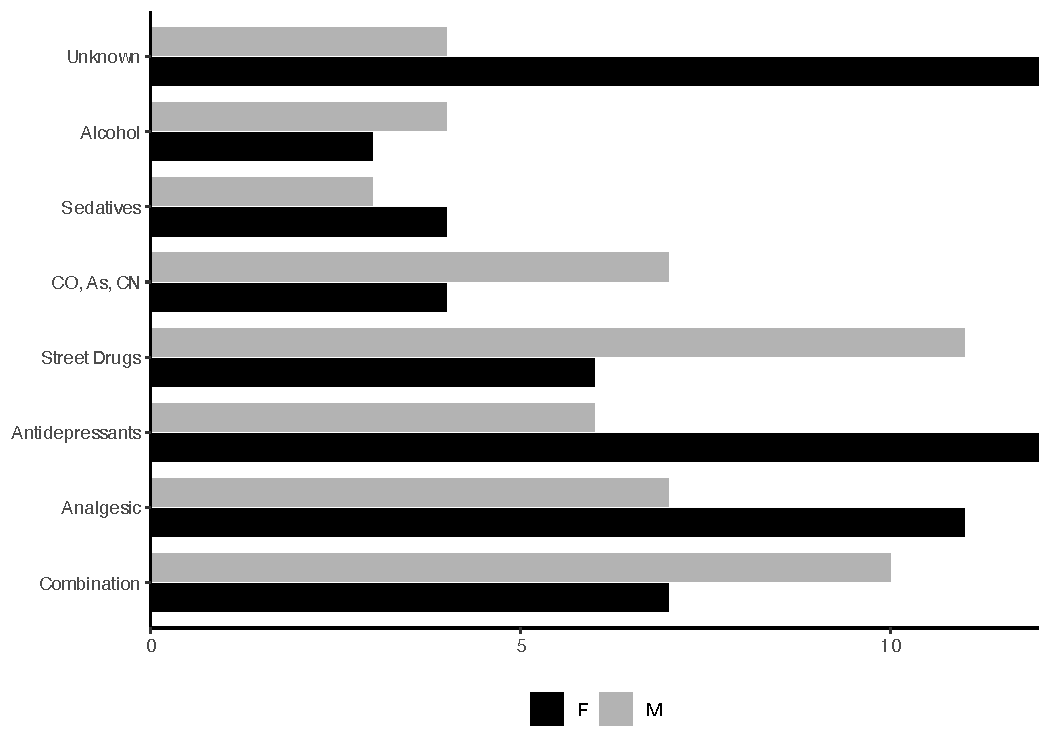
\includegraphics[width=0.9\linewidth]{../../notebook/yash/fig_1} \caption{Females show relatively higher counts in analgesic and antidepressant exposures, whereas males are more represented in CO/As/CN and street drug exposures. These differences are not statistically significant.}\label{fig:fig1}
\end{figure}

\begin{figure}
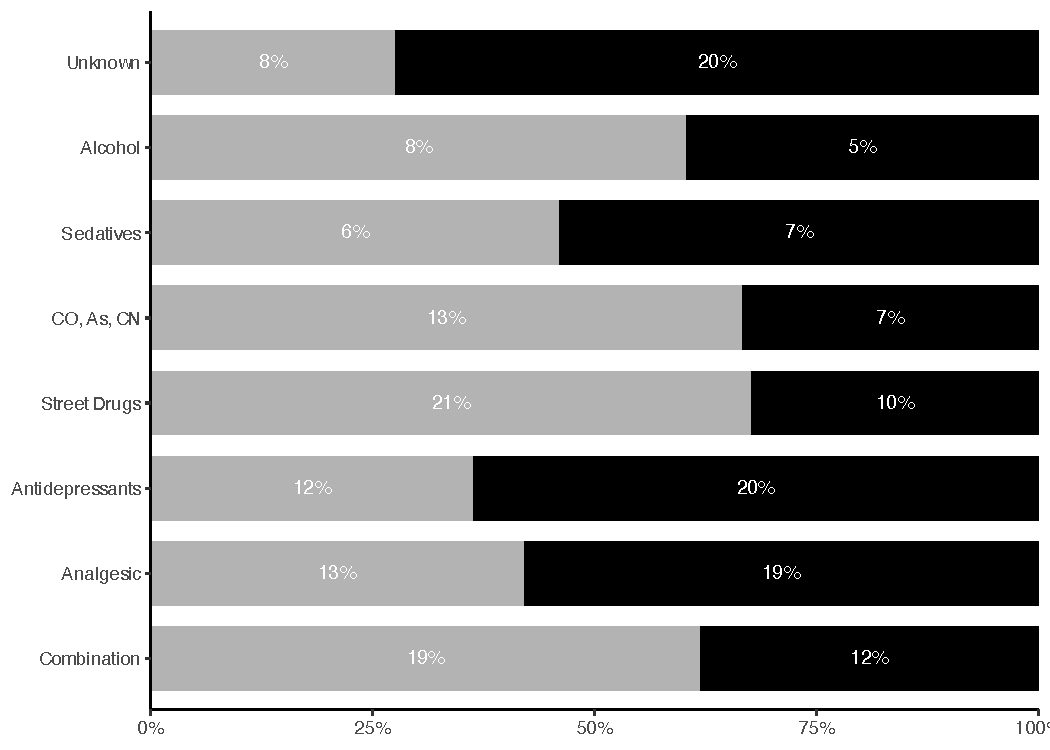
\includegraphics[width=0.9\linewidth]{../../notebook/yash/fig2} \caption{Within-gender proportions for each exposure category (bars sum to 100\% for each gender). Females have higher proportions in analgesic and antidepressant exposures, while males show higher proportions in CO/As/CN and street drugs. The chi-square test indicates the overall gender–exposure association is not statistically significant.}\label{fig:fig2}
\end{figure}

\end{document}
